\documentclass[specialist, substylefile = spbu.rtx,
			   subf, href, 12pt]{disser}
			   
\usepackage[a4paper, includefoot,
			left=3cm, right=1.5cm,
			top=2cm, bottom=2cm,
			headsep=1cm, footskip=1cm]{geometry}

\usepackage{cmap}
\usepackage[T2A]{fontenc}
\usepackage[utf8]{inputenc}
\usepackage[english,russian]{babel}
\usepackage{amssymb, amsfonts, amsmath, amsthm} % математические дополнения от АМС
\usepackage{graphicx}

% Включать подсекции в оглавление
\setcounter{tocdepth}{2}

\graphicspath{{images/}{code_snippets/}}
\DeclareGraphicsExtensions{.png,.jpg}

\newcommand\eqdef{\mathrel{\stackrel{\makebox[0pt]{\mbox{\normalfont\tiny def}}}{=}}}



\begin{document}

\institution{%
	Санкт-Петербургский государственный университет\\
	Прикладная математика и информатика
}

\title{Учебная практика 2 (проектно-технологическая) (семестр 3)}

% Тема
\topic{Обнаружение разладки с помощью метода SSA}

% Автор
\author{Кононыхин Иван Александрович}
\group{группа 20.М03-мм}

% Научный руководитель
\sa       {Голяндина Нина Эдуардовна\\%
	Кафедра статистического моделирования}
\sastatus {к.\,ф.-м.\,н., доцент}

% Город и год
\city{Санкт-Петербург}
\date{2021}

\maketitle



\newpage
\tableofcontents
\newpage

\intro
Будем называть временной ряд $F_N = (f_1, \cdots, f_{N})$ \textbf{однородным}, если он управляется некоторым линейным рекуррентным соотношением $(LRR)$ $f_{n+r} = \sum_{i=1}^{r} \alpha_i\cdot f_{n+r-i}, \; \alpha_i \neq 0$, размерность которого ($r$) мала по отношению к $\mathrm{N}$. 

Предположим, что из-за внешнего воздействия (или по другой причине) однородный временной ряд подвергается мгновенному возмущению, то есть он перестает следовать исходному $\mathrm{LRR}$. Однако по прошествии определенного периода времени он снова становится управляемым неким $\mathrm{LRR}$, которое может отличаться от исходного. В результате, ряд в целом перестает быть однородным и возникает проблема изучения этой неоднородности.

Метод, основанный на алгоритме SSA (Singular Spectrum Analysis) \cite{TSStructure}, позволяет изучить эту неоднородность путем построения матрицы разладки, где для обнаружения неоднородности используются строковые, столбцовые и диагональные подмножества этой матрицы.

Целью данной работы является сравнение методов обнаружения неоднородности в синусоидальных рядах, а также расширение существующего функционала в задаче обнаружения разладки в режиме реального времени.

В <<Главе 1>> приведена теория базового алгоритма SSA.

В <<Главе 2>> введены коэффициент неоднородности, матрица разладки, функции обнаружения и обозреваются типы неоднородности.

В <<Главе 3>> посвящена сравнению функций обнаружения неоднородностей на синусоидальных временных рядах с шумом и без. Неоднородность рядов задавалась изменением частоты, амплитуды, фазовым сдвигом и выбросом.

<<Глава 4>> посвящена аналитическому анализу индекса неоднородности, его упрощению и аналитической аппроксимацией. Приведены тесты подтверждающие эквивалентность новой формулы и старой.


\newpage
\chapter{Singular spectrum analysis}
\section{Алгоритм базового метода SSA}
Определим метод SSA как любой метод, состоящий из четырех этапов, описанных ниже. Обозначим входной объект как $F_N$ --- упорядоченный набор из $\mathrm{N}$ действительных чисел (временной ряд).

\subsection{Вложение}
\label{step:Embedding}

Процедура вложения переводит исходный временной ряд $F_N = (f_1, \dotsc, f_{N})$ в последовательность многомерных векторов 
$$X_i = (f_{i}, \dotsc, f_{i+L-1})^\mathrm{T}, \;\;\; 1 \leq i \leq K$$
размерности $L$ (длина окна), где $K = N - L + 1$. 

Создается траекторная матрица $\bold{X} = [X_1, \dotsc, X_K]$ размерности $L \times K$, имеющую Ганкелеву структуру с одинаковыми значениями на анти-диагоналях
$$\bold{X} =
\begin{pmatrix}
		f_{1} & f_{2} & f_{3} & \ldots & f_{K}\\
		f_{2} & f_{3} & f_{4} & \ldots & f_{K+1}\\
		f_{3} & f_{4} & f_{5} & \ldots & f_{K+2}\\
		\vdots & \vdots & \ddots & \vdots\\
		f_{L} & f_{L+1} & f_{L+2} & \ldots & f_{N}
\end{pmatrix}.
\eqno{(1.1)}
$$

\subsection{Сингулярное разложение}

Результатом этого шага является сингулярное разложение траекторной матрицы $\bold{X}$. 

Пусть $\bold{S} = \bold{X}\bold{X}^\mathrm{T}$, $\lambda_1 \geq \dotsc \geq \lambda_L \geq 0$ - собственные числа матрицы $\bold{S}$, $d = rank\;\bold{X} = max\{j\;:\;\lambda_j > 0\}$, $U_1, \dotsc, U_d$ - ортонормированный набор собственных векторов матрицы $\bold{S}$, соответствующий собственным числам, и $V_j = \bold{X}^\mathrm{T}U_j/\sqrt{\lambda_j}, j = 1, \dotsc, d$ - факторные векторы. Тогда разложение будет иметь вид
$$\bold{X} = \sum\limits_{i=1}^{d}\bold{X}_i, \;\;\; \bold{X}_i = \sqrt{\lambda_i}U_iV_i^\mathrm{T}. \eqno{(1.2)}$$

\subsection{Группировка}

На основе разложения шага 2 процедура группировки делит множество индексов $\{1, \dotsc, d\}$ на $m$ непересекающихся подмножеств $I_1, \dotsc, I_m$.

Пусть $I = \{i_1, \dotsc, i_p\} \subset \{1, \dotsc, d\}$ - набор индексов. Тогда результирующая матрица $\bold{X}_I$, соответствующая группе $I = \{i_1, \dotsc, i_p\}$ определяется как 
$$\bold{X_I} = \bold{X}_{i_1} + \dotsc + \bold{X}_{i_p}.$$
Такие матрицы вычисляются для $I = \{I_1, \dotsc, I_m\}$, тем самым, разложение $(1.2)$ может быть записано в сгруппированном виде
$$\bold{X} = \bold{X}_{I_1} + \dotsc + \bold{X}_{I_m}. \eqno{(1.3)}$$

\subsection{Реконструкция}

На последнем шаге базового алгоритма каждая матрица сгруппированного разложения $(1.3)$ преобразуется в новый ряд длины $N$ диагональным усреднением элементов.

Пусть $Y$ --- матрица $L \times K$ с элементами $y_{ij}$, где $1 \leq i \leq L,\; 1 \leq j \leq K$. Обозначим $L^* = \min(L, K), \; K^* = \max(L, K)$. Пусть $y_{ij}^* = y_{ij}$ если $L<K$ и $y_{ij}^* = y_{ji}$ в противном случае. Диагональное усреднение преобразует матрицу $Y$ в ряд $g_0, \dotsc, g_{N-1}$ по формуле
$$g_k = 
	\begin{cases}
		\frac{1}{k+1}\sum\limits_{m=1}^{k+1}y_{m, k-m+2}^* & 0 \leq k < L^* -1, \\\
		\frac{1}{L^*}\sum\limits_{m=1}^{L^*}y_{m, k-m+2}^* & L^* - 1 \leq k < K^*, \\\
		\frac{1}{N-k}\sum\limits_{m=k - K^* + 2}^{N - K^* + 1}y_{m, k-m+2}^* & K^* \leq k < N.
	\end{cases}
\eqno{(1.4)}$$

Применяя диагональное усреднение $(1.4)$ к результирующим матрицам $\bold{X_{I_k}}$, получаем $m$ рядов $\widetilde{F}_{k} = (\widetilde{f}_0^{(k)}, \dotsc, \widetilde{f}_{N-1}^{(k)})$. Тогда исходный ряд $F_N$ раскладывается в сумму рядов:
$$F_N = \sum\limits_{k=1}^{m}\widetilde{\mathbb{X}}_k.$$

\section{Ранги ряда}
Рассмотрим ряд $F_N = (f_1,\cdots,f_N)$. После процедуры вложения мы получаем подряды длины $L:\; X_i^{(L)} = X_i = (f_{i}, \cdots, f_{i+L-1})^\mathrm{T}, \; 1 \leq i \leq K,$ $\mathfrak{L}^{(L)} = \mathfrak{L}^{(L)}(F_N) \eqdef \mathrm{span}(X_1, \cdots, X_K)$ --- траекторное пространство ряда $F_N$.

Будем говорить, что ряд имеет ранг $d$, если $\dim\mathfrak{L}^{(L)} = d$ и записывать это как $\textrm{rank}_L(F_N) = \textrm{rank}(\bold{X}) = \textrm{rank}(\bold{XX}^\mathrm{T}) = \textrm{rank}(\bold{X}^\mathrm{T}\bold{X}) = d$. Справедливым равенство будет в том случае, если $d\leq\min(L, K)$. Если же равенство $\textrm{rank}_L(F_N) = d < \frac{N}{2}$ будет достигаться $\forall$ допустимого $L$, то говорим, что ряд $F_N$ имеет ранг $d$ ($\textrm{rank}(F_N) = d$) и при существовании такого $d$ ряд $F_N$ --- ряд конечного ранга.

Если же мы рассмотрим бесконечный временной ряд $F=(\cdots, f_{-1}, f_0, f_1, \cdots)$, то такой ряд будем называть рядом конечного ранга тогда и только тогда, когда он управляется LRR размерности $d$, то есть существуют такие $\alpha_1, \cdots, \alpha_d \; \forall n: \; f_{n+r} = \sum_{i=1}^{r} \alpha_i\cdot f_{n+r-i}, \; \alpha_i \neq 0$.

\subsection{Пример}

Рассмотрим ряд $F_N = C\sin(2\pi\omega n + \phi),\;\phi \in [0, 2\pi), \; \omega \in [0, \frac{1}{2}]$. Если $\omega < \frac{1}{2}$, то $\forall L\geq 2$ и $N\geq L+1$ сингулярное разложение траекторной матрицы имеет 2 члена (то есть ранг равен 2). При $\omega=\frac{1}{2}$ ранг равен $1$. Отсюда, на практике при SSA разложении в такого вида рядах (где сигнал задан синусом) даже при наличии шума, в качестве количества рассматриваемых собственных векторов указывают $r=2$, что соответствует компонентам сигнала.

\chapter{Поиск разладки}
Основная идея метода решения задачи обнаружения структурных изменений может быть описана следующим образом. Временной ряд $F_N$, управляемый LRR, характеризуется тем, что для достаточно больших значений длины окна $L$ (Гл. \ref{step:Embedding}) (это значение должно быть больше размерности минимального LRR) вложенные векторы покрывают одно и то же линейное пространство $\mathfrak{L}^{(L)}$ независимо от $N$ (если $N$ достаточно велико). Таким образом, нарушения однородности ряда могут быть описаны в терминах соответствующих сдвинутых векторов: возмущения заставляют эти векторы покидать пространство $\mathfrak{L}^{(L)}$. Соответствующие расхождения определяются в терминах расстояний между сдвинутыми векторами и пространством $\mathfrak{L}^{(L)}$, которые могут быть определены для различных частей ряда (например, до и после возмущения).

\section{Матрица неоднородности и функции неоднородности}
\subsection{Матрица неоднородности}

Рассмотрим два временных ряда $F^{(1)} = F_{N_1}^{(1)}$ и $F^{(2)} = F_{N_2}^{(2)}$ и зададим число $L: 2 \leq L \leq \min(N_1 - 1, N_2)$. Обозначим $\mathfrak{L}^{(L, 1)}$ линейное пространство, натянутое на $L$---сдвинутые векторы ряда $F^{(1)}$.

Пусть $ U_l^{(1)} (l = 1, \dotsc, L) $ --- левые сингулярные векторы траекторной матрицы ряда $ F^{(1)} $. Для $ l > d \eqdef dim \; \mathfrak{L}^{(L, 1)}$ в качестве собственных векторов $ U_l^{(1)} $ мы берем векторы из любого ортонормированного базиса пространства, ортогонального $\mathfrak{L}^{(L, 1)}$.

Пусть $ I = \{i_1, \dotsc, i_r\} $ --- подмножество $ \{1, \dotsc, L\} $ и $ \mathfrak{L}_r^{(1)} \eqdef span(U_l^{(1)}, l \in I) $. Обозначим через $ X_1^{(2)}, \dotsc, X_{K_2}^{(2)} (K_2 = N_2 - L + 1) $ $L$-сдвинутые векторы временного ряда $F^{(2)}$.

Введем меру, называемую \textbf{индексом неоднородности}, которая характеризует несоответствие между рядом $F^{(2)}$ и структурой ряда $F^{(1)}$ (описываемого подпространством $ \mathfrak{L}_r^{(1)} $):
$$g(F^{(1)}; F^{(2)}) = \frac{\sum\limits_{l=1}^{K_2}\mathrm{dist}^2(X_l^{(2)}, \mathfrak{L}_r^{(1)})}{\sum\limits_{l=1}^{K_2}\|X_l^{(2)}\|^2} = \frac{\sum\limits_{l=1}^{K_2}\;(\|X_l^{(2)}\|^2 - \sum\limits_{i=1}^{r}\langle X_l^{(2)}, U_i^{(1)}\rangle^2)}{\sum\limits_{l=1}^{K_2}\|X_l^{(2)}\|^2} = 1 - \frac{\sum\limits_{l=1}^{K_2}\;\sum\limits_{i=1}^{r}\langle X_l^{(2)}, U_i^{(1)}\rangle^2}{\sum\limits_{l=1}^{K_2}\|X_l^{(2)}\|^2} . \eqno{(2.1)}$$
Значения $g$ принадлежат интервалу $[0, 1]$.

Введем обозначения:
\begin{enumerate}
	
	\item
	Исходный временной ряд $ F_N: F_N = (f_0, \dotsc, f_{N - 1}), N > 2 $;
	
	\item
	Подряды (интервалы) $ F_{i, j} $ временного ряда $ F_N: F_{i, j} = (f_{i - 1}, \dotsc, f_{j - 1}), \; 1 \leq i < j \leq N $;
	
	\item
	Длина окна $ L: \; 1 < L < N $;
	
	\item
	Длина $ B $ базовых подрядов ряда $ F_N: B > L $;
	
	\item
	Длина $ T $ тестовых подрядов ряда $ F_N: T \geq L $;
	
	\item
	Предполагаем набор $ I = \{j_1, \dotsc, j_r\} $ различных натуральных чисел: $ j < \min(L, B - L + 1) $ $ \forall $ $ j \in I $.
	
	\item
	Базовые пространства $ (i = 1, \dotsc, N - B + 1) $ натянуты на собственные векторы с индексами из $ I $, полученные сингулярным разложением траекторных матриц $ \mathbf{X}^{(i, B)} $ ряда $ F_{i, i+B-1} $ с длиной окна $ L $. Соответствующий набор собственных троек называется \textbf{базовым набором собственных троек}.
	
\end{enumerate}

Учитывая эти обозначения, матрица $ \mathbf{G} = \mathbf{G}_{B, T} $, состоящая из элементов $g_{ij}$:
$$g_{ij} = g(F_{i, i+B-1};\;F_{j, j+T-1}), \eqno{(2.2)}$$ 
$$1 \leq i \leq N-B+1,\;\;\;\;\; 1 \leq j \leq N-T+1,$$
есть \textbf{матрица неоднородности} $ (\mathrm{H}-matrix) $ временного ряда $ F_N $. Отсюда следует, что пространство $ \mathfrak{L}_{I, B}^{(L, i)} $ соответствует пространству $ \mathfrak{L}_r^{(1)} $. Ряд $ F_{i, i+B-1} $ называют \textbf{базовым подрядом} (или базовым интервалом), а $ F_{j, j+T-1} $ --- \textbf{тестовым подрядом} (интервалом). По определению, величина $g_{ij}$ является нормированной суммой расстояний между $L$-сдвинутыми векторами тестового подряда и линейным пространством $ \mathfrak{L}_{I, B}^{(L, i)} $. 

\subsection{Функции обнаружения}
На основе матрицы неоднородности $ \mathbf{G} $ введем различные функции обнаружения.

\begin{enumerate}
	\item
	Строковая функция обнаружения
	
	Строковой функцией обнаружения является ряд $ D_{T,N}^{(r)} $ c членами, определяемыми
	$$ d_{n-1}^{(r)} \eqdef g(F_{1, B};\; F_{n-T+1, n}), \;\; T \leq n \leq N,  \eqno{(2.3)} $$
	что соответствует обнаружению изменений по отношению к начальной части ряда (или, точнее, к его первым $ B $ членам, которые представлены пространством $ \mathfrak{L}_{I, B}^{(L, 1)} $).
	
	\item
	Столбцовая функция обнаружения
	
	Столбцовой функцией обнаружения является ряд $ D_{B,N}^{(c)} $ c членами, определяемыми
	$$ d_{n-1}^{(c)} \eqdef g(F_{n-B+1, n};\; F_{1, T}), \;\; B \leq n \leq N.  \eqno{(2.4)} $$
	
	\item
	Функция диагонального обнаружения
	
	Функцией диагонального обнаружения является ряд $ D_{T+B,N}^{(d)} $ c членами, определяемыми
	$$ d_{n-1}^{(d)} \eqdef g(F_{n-T-B+1, n-T+1};\; F_{n-T+1, n}), \eqno{(2.5)} $$
	$$T + B \leq n \leq N.$$
	
	Поскольку промежуток между базовым и тестовым интервалами отсутствует, данная функция обнаружения может использоваться для обнаружения резких структурных изменений на фоне медленных.
	
	\item
	Функция симметричного обнаружения
	
	Пусть $ T = B $. Функцией симметричного обнаружения является ряд $ D_{B,N}^{(s)} $ c членами, определяемыми
	$$ d_{n-1}^{(s)} \eqdef g(F_{n-B+1, n};\; F_{n-B+1, n}), \;\; B \leq n \leq N.  \eqno{(2.6)} $$
	
	Эта функция обнаружения измеряет качество приближения базового ряда выбранными собственными тройками.
	
\end{enumerate}

\section{Однородность и неоднородность}

Пусть $ F_N $ --- однородный временной ряд, управляемый минимальным $ \mathrm{LRR} $ размерности $ d $. Выберем $ L $ и $ r $ такие, что $ L \geq d, \; d \leq r \leq \min(L, N-L+1)$.

Если выбрать $ I = \{1, \dots, r\} $, то матрица неоднородности $ (2.1) $ будет нулевой, поскольку $ B \geq L $, $ \forall \; i \; \mathfrak{L}^{(L)}(F_{i, i+B-1}) = \mathfrak{L}^{(L)}(F_N) $, следовательно, все $ L $-сдвинутые векторы ряда $ F_{j, j+T-1} $ лежат в пространстве $ \mathfrak{L}^{(L)}(F_{i, i+B-1}) \; \forall \; i,\; j $. Это означает, что любой однородный ряд $ F_N $ порождает нулевую матрицу неоднородности, а наличие ненулевых элементов $ g_{ij} $ в этой матрице свидетельствует о нарушении однородности.

Рассмотрим несколько типов нарушений.

\subsection{Типы неоднородности}

Как указывалось ранее, временной ряд $ F_N $ задан $ \mathrm{LRR} $ до определенного времени $ Q $. Затем происходит мгновенное возмущение, хотя через короткое время ряд снова становится однородным и подчиняется $ \mathrm{LRR} $, которое может отличаться от исходного.

Если начальное $ \mathrm{LRR} $ восстанавливается, то мы имеем \textbf{временное} нарушение структуры временного ряда. В противном случае нарушение является \textbf{постоянным}.

Момент времени $ Q $ будем называть \textbf{моментом возмущения} или \textbf{точкой изменения}. Положим $ d = \mathrm{rank}_L(F_{1, Q-1}) $.

Предположим, что через некоторое время $ S \geq 0 $ после возмущения, временной ряд стал опять однородным (ряд $ F_{Q+S, N} $). Обозначим $ d_1 = \mathrm{rank}_L(F_{Q+S, N}) $. Временной интервал $ [Q, Q + S] $ называется \textbf{переходным интервалом} (поведение ряда на котором нас не интересует).

Пусть $ L \geq \max(d, d_1) $. Дополнительно введем ограничения $ L \leq Q-1 $ и $ L \leq N-Q-S+1 $. Если $ L $-сдвинутые векторы ряда $ F_N $ покрывают исходное подпространство $ \mathfrak{L}^{(L)}(F_{1, Q-1}) $ после того, как они покинули переходный интервал (то есть  $ \mathfrak{L}^{(L)}(F_{1, Q-1}) = \mathfrak{L}^{(L)}(F_{Q+S, N})$), тогда обе однородные части временного ряда соответствуют одному минимальному $ \mathrm{LRR} $ --- случай временной неоднородности. Отсюда вытекает случай постоянной неоднородности.

Опишем вид матрицы неоднородности. Пусть длины базового и тестового интервалов удовлетворяют условию $ \max(B, T) < Q $. Предположим, что $ I = \{1, \dots, r\} $ и $ r = d \leq \min(L, B-L+1) $. Тогда все элементы $ g_{ij} $ матрицы $ \mathbf{G}_{B, T} $ равны нулю для $ i+B \leq Q $ и $ j+T \leq Q $. Это связано с тем, что для этих индексов, и базовый, и тестовый подряды исходного ряда $ F_N $ также являются подрядами однородного ряда $ F_{1, Q-1} $. Значения остальных элементов матрицы неоднородности зависят от типа неоднородности и значений параметров.

Схематично, общая форма матрицы неоднородности изображена на Рис. 2.1. 

Регион $ \mathcal{A} $ соответствует элементам $ g_{ij} $ где ряды $ F_{i, i+B-1} $ и $ F_{j, j+T-1} $ являются подрядами однородного ряда $ F_{1,Q-1} $. Отсюда следует, что данный регион состоит из нулевых элементов. 

В регионе $ \mathcal{D} $ те же самые ряды являются подрядами ряда $ F_{Q+S,N} $. Поэтому, если размерность $ d_1 $ ряда $ F_{Q+S, N} $ не больше размерности $ d $ ряда $ F_{1, Q-1} $, то данный регион матрицы также состоит из нулевых элементов.


\begin{figure}[h]
	\center{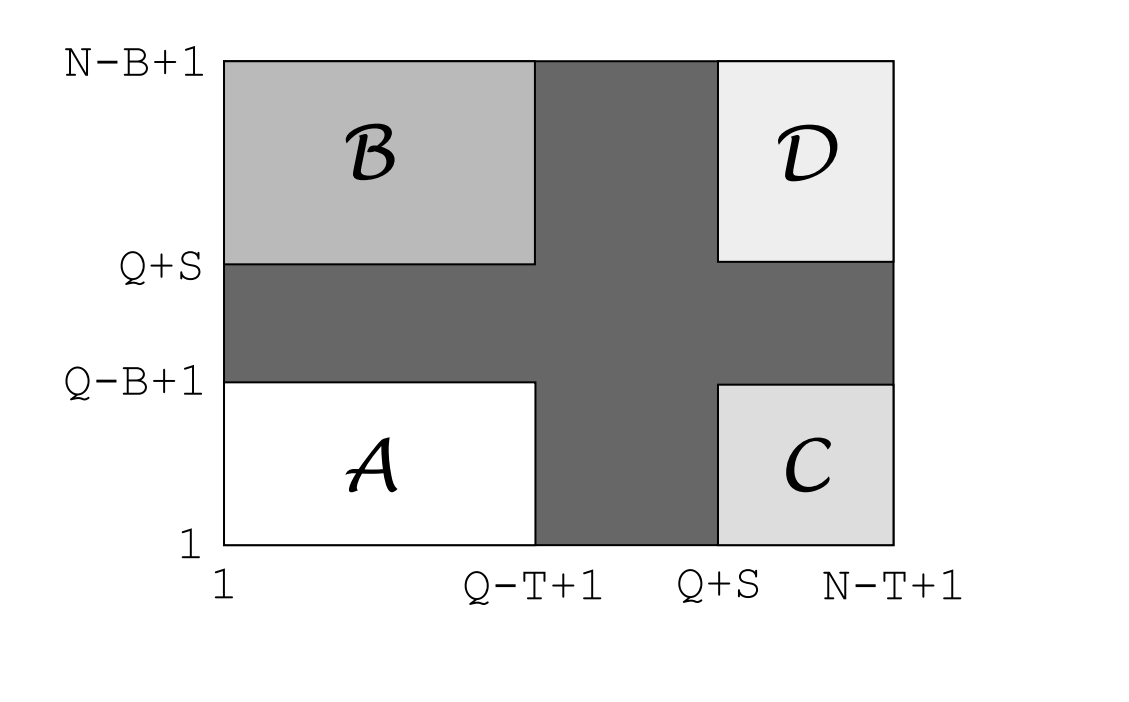
\includegraphics[width=0.7\linewidth]{2.1}}
	\caption{Общая форма матрицы неоднородности.}
\end{figure}

\textbf{Крест неоднородности} --- регион в матрице неоднородности с индексами элементов
$$Q-B+1 \leq i \leq Q+S-1, \;\;\; Q-T+1 \leq j \leq Q+S-1.$$
Эти элементы соответствуют тому, что либо тестовый интервал, либо базовый имеет пересечение с переходным.

\newpage
\chapter{Сравнение функций разладки}

Так как у нас есть четыре функции обнаружения неоднородности:
\begin{enumerate}
	\item 
	Строковая: $d_{n-1}^{(r)} \eqdef h_{b-T}^{(r, 1)} = g(F_{1, B};\; F_{n-T+1, n}), \;\; T \leq n \leq N.$
	
	\item
	Столбцовая: $d_{n-1}^{(c)} \eqdef h_{n-B}^{(1, c)} = g(F_{n-B+1, n};\; F_{1, T}), \;\; B \leq n \leq N.$
	
	\item
	Диагональная: $d_{n-1}^{(d)} \eqdef h_{n-T-B}^{(d, B)} = g(F_{n-T-B+1, n-T+1};\; F_{n-T+1, n}), T + B \leq n \leq N.$
	
	\item
	Симметричная: $d_{n-1}^{(s)} \eqdef h_{n-B}^{(s)} = g(F_{n-B+1, n};\; F_{n-B+1, n}), \;\; B \leq n \leq N.$
	
\end{enumerate}
можем экспериментальным путем попытаться определить, какая из них лучше обнаруживает разладку в ряде.

\section{Постановка задачи}
Рассмотрим ряд $$f_n = 
\begin{cases}
	C_1\sin(2\pi\omega_1n + \phi_1), & n < Q, \\
	C_2\sin(2\pi\omega_2n + \phi_2), & n \geq Q,
\end{cases}$$
чьи параметры буду задаваться типом разладки и соответствующим изменением параметров.
Рассмотрим два типа неоднородности:
\begin{enumerate}
	\item
	Временную, заданную
	\begin{enumerate}
		\item 
		Фазовым сдвигом: $\phi_1 \neq \phi_2$;
		\item 
		Выбросом:
		$$f_n = 
		\begin{cases}
			C_1\sin(2\pi\omega_1n + \phi_1) & n \neq Q, \\
			10\cdot C_1 & n = Q.
		\end{cases}$$
		\item 
		Изменением амплитуды: $C_1 \neq C_2$.
	\end{enumerate}
	
	\item
	Постоянную, заданную
	\begin{enumerate}
		\item 
		Изменением частоты: $\omega_1 \neq \omega_2$.
	\end{enumerate}
	
\end{enumerate}

Ряды, заданные параметрами выше, порождают матрицы неоднородности, изображенные на Рис. \ref{pic:heterogeneity_types}
\begin{figure}[!hhh]
	\center{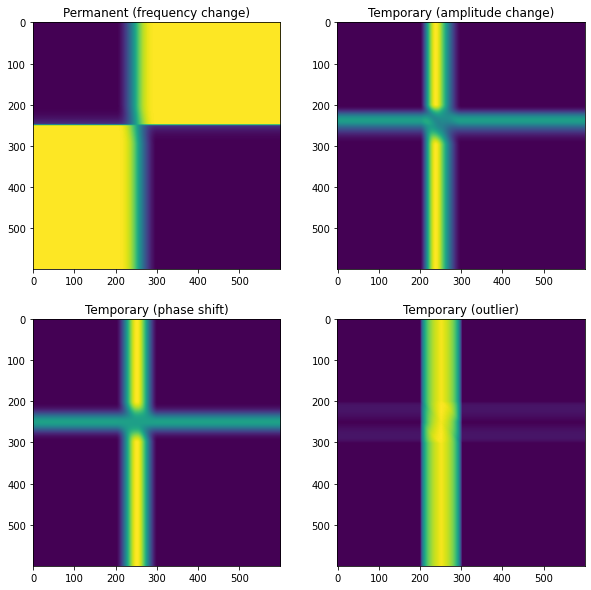
\includegraphics[width=1\linewidth]{heterogeneity_types}}
	\caption{Временные ряды без шума.}
	\label{pic:heterogeneity_types}
\end{figure}


В качестве оценок функций неоднородности будем учитывать скорость возрастания значений и момент преодоления $n_{overcome}$ заданного порога $\delta$.


\section{Экспериментальные установки}
Для реализации тестов был выбран язык $Python3$. Взаимодействие с пакетом $RSSA$ осуществлялось через библиотеку $rpy2$ (стадии вложения и сингулярного разложения). Подсчет индексов неоднородности велись функционалом языка $Python3$ и библиотеку $numpy$. Работа с графикой велась через библиотеку $matplotlib$. 

Параметры ряда были заданы следующим образом: 

$ N = 700, \;\omega_1 = \frac{1}{10},\; \omega_2 = \frac{1}{5},\; C_1 = 1, \; C_2 = 2,\; \phi_1=0,\; \phi_2=\frac{\pi}{2},\; Q = 301,\; B = T = 100,\; L = 50,\; r=d=rank(f_n)=2$.

В тестах предполагаем, что момент разладки $Q$ известен и для оценки скорости возрастания будем выводить значения функций в точках $[Q, Q+10, Q+20, Q+30]$.

Порог, относительно которого будем определять, какая из функций неоднородности раньше обнаруживает разладку зададим в  соответствии с промоделированными значениями, описанными ниже.

\section{Моделирование}
Для определения момента преодоления значения порога $\delta$ необходимо этот порог задать. Для этого к рассмотренным рядам добавим шум $\epsilon\sim N(0, \sigma^2)$, где $\sigma = 0.5$. Для ряда с временной разладкой, заданной изменением амплитуды ($C_1 \neq C_2$), зададим дисперсию шума до разладки как $\frac{\sigma^2}{2}$, чтобы шум $\epsilon$ был пропорционален амплитуде ряда, так как в противном случае, сила шума не позволит корректно определить базис пространства $ \mathfrak{L_r} $. 

Промоделируем реализации шума $n_{mod}=200$ раз и посчитаем такие характеристики ряда на промежутке $[0, \cdots, Q-1]$, как средний максимум и $95$-й процентиль. Эти два значения возьмем в качестве параметра $\delta$. 

Результаты моделирования представлены в таблице \ref{tab:ModellingResults}.
\begin{table}[!hhh]
	\center
	\caption{Значения моделирования.}
	\begin{tabular}{lllll}
	    Permanent ($\omega_1 \neq \omega_2$) & row & col & sym & diag \\
	    meanMax & 0.2391 & 0.2062 & 0.2339 & 0.2185 \\
	    95 procentile & 0.2352 & 0.2054 & 0.2297 & 0.2167 \\
	    &  &  &  &  \\
	    Temporary ($C_1 \neq C_2$) & row & col & sym & diag \\
	    meanMax & 0.0685 & 0.0593 & 0.0669 & 0.0624 \\
	    95 procentile & 0.0673 & 0.0591 & 0.0657 & 0.0616 \\
	    &  &  &  &  \\
	    Temporary ($\phi_1 \neq \phi_2$) & row & col & sym & diag \\
	    meanMax & 0.2372 & 0.2044 & 0.2319 & 0.2166 \\
	    95 procentile & 0.2336 & 0.2036 & 0.2279 & 0.2143 \\
	    &  &  &  &  \\
	    Temporary (Outlier) & row & col & sym & diag \\
	    meanMax & 0.2336 & 0.2069 & 0.2287 & 0.2161 \\
	    95 procentile & 0.2307 & 0.2061 & 0.2254 & 0.2139
	\end{tabular}
\label{tab:ModellingResults}
\end{table}


\newpage

\subsection{Ряды без шума}

Временные ряды и их функции неоднородности изображены на Рис. \ref{pic:TimeSeriesWithoutNoise} и Рис. \ref{pic:HeterFuncsWithoutNoise} соответственно.


Полученные результаты тестирования функций разладки приведены в таблицах \ref{tab:PermanentHeterogeneity}, \ref{tab:TemporaryHeterogeneityAmplitude}, \ref{tab:TemporaryHeterogeneityShifted}, \ref{tab:TemporaryHeterogeneityOutlier}.

\newpage
\begin{figure}[!hhh]
	\center{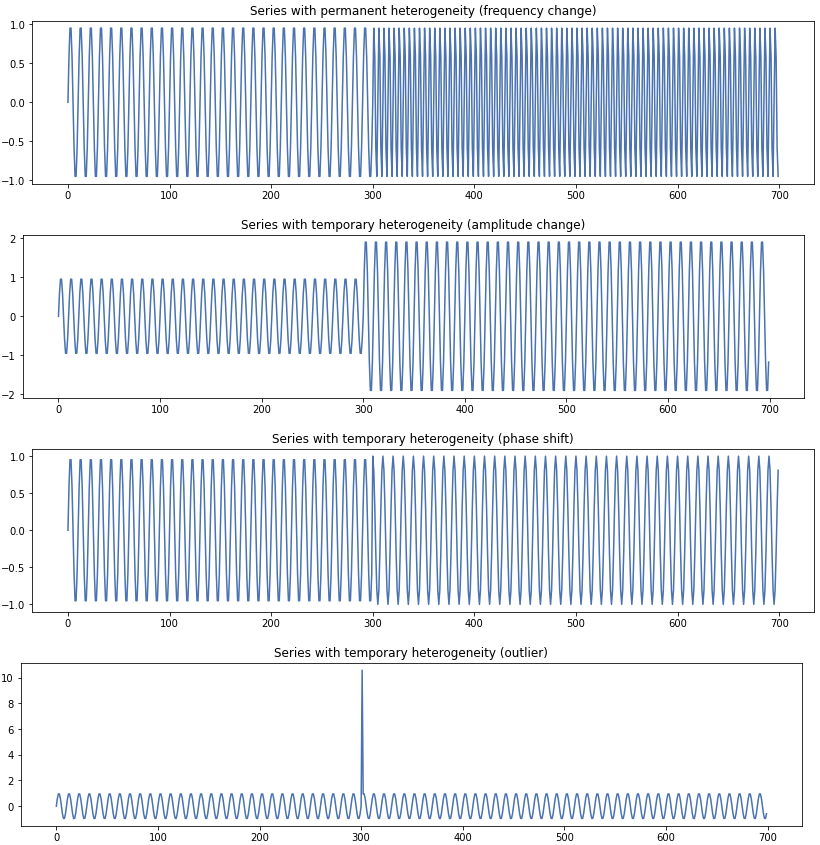
\includegraphics[width=1\linewidth]{seriesTests}}
	\caption{Временные ряды без шума.}
	\label{pic:TimeSeriesWithoutNoise}
\end{figure}

\newpage
\begin{figure}[!hhh]
	\center{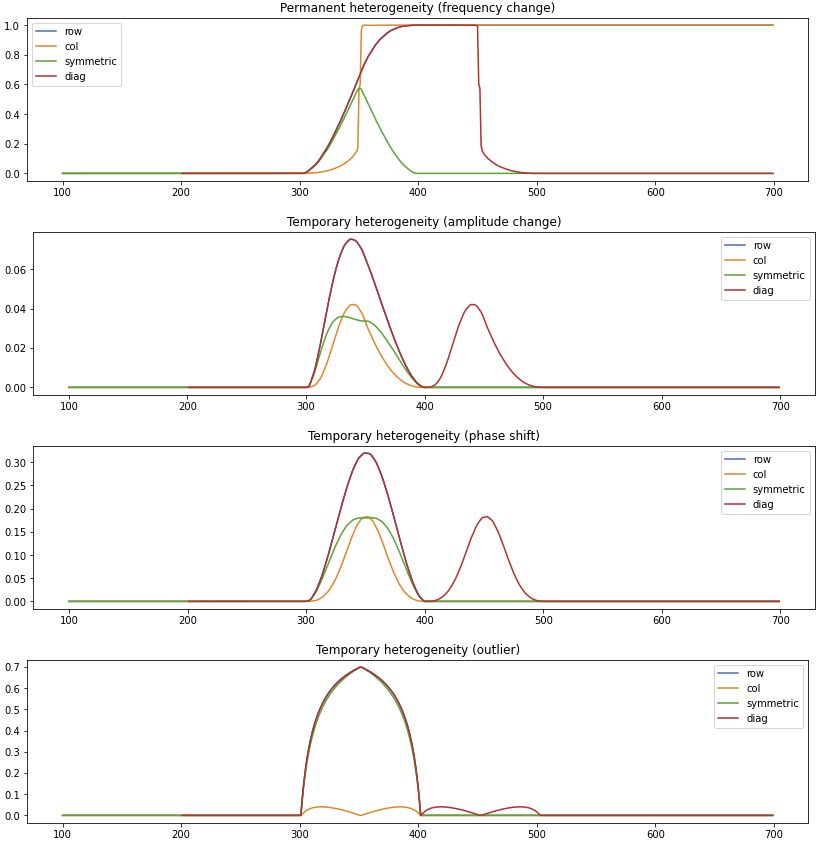
\includegraphics[width=1\linewidth]{detectionTests}}
	\caption{Функции неоднородности рядов без шума.}
	\label{pic:HeterFuncsWithoutNoise}
\end{figure}


\newpage
\begin{table}[!hhh]
	\caption{Характеристики функций неоднородности для постоянной разладки ($\omega_1 \neq \omega_2$).}
	\begin{tabular}{lllllll}
		Row & meanMax & 95 procentile &  & Col & meanMax & 95 procentile \\
		$n_{overcome}$ & 328 & 328 &  & $n_{overcome}$ & 350 & 350 \\
		$D_Q^{(r)}$ & 0.0000 & 0.0000 &  & $D_Q^{(c)}$ & 0.0000 & 0.0000 \\
		$D_{Q+10}^{(r)}$ & 0.0428 & 0.0428 &  & $D_{Q+10}^{(c)}$ & 0.0028 & 0.0028 \\
		$D_{Q+20}^{(r)}$ & 0.1468 & 0.1468 &  & $D_{Q+20}^{(c)}$ & 0.0140 & 0.0140 \\
		$D_{Q+30}^{(r)}$ & 0.2962 & 0.2962 &  & $D_{Q+30}^{(c)}$ & 0.0385 & 0.0385 \\
		&  &  &  &  &  &  \\
		Sym & meanMax & 95 procentile &  & Diag & meanMax & 95 procentile \\
		$n_{overcome}$ & 329 & 329 &  & $n_{overcome}$ & 327 & 327 \\
		$D_Q^{(s)}$ & 0.0000 & 0.0000 &  & $D_Q^{(d)}$ & 0.0000 & 0.0000 \\
		$D_{Q+10}^{(s)}$ & 0.0402 & 0.0402 &  & $D_{Q+10}^{(d)}$ & 0.0428 & 0.0428 \\
		$D_{Q+20}^{(s)}$ & 0.1354 & 0.1354 &  & $D_{Q+20}^{(d)}$ & 0.1468 & 0.1468 \\
		$D_{Q+30}^{(s)}$ & 0.2706 & 0.2706 &  & $D_{Q+30}^{(d)}$ & 0.2962 & 0.2962
	\end{tabular}
	\label{tab:PermanentHeterogeneity}
\end{table}

\begin{table}[!hhh]
	\caption{Характеристики функций неоднородности для временной разладки ($ C_1 \neq C_2 $).}
	\begin{tabular}{lllllll}
		Row & meanMax & 95 procentile &  & Col & meanMax & 95 procentile \\
		$n_{overcome}$ & 330 & 330 &  & $n_{overcome}$ &  &  \\
		$D_Q^{(r)}$ & 0.0000 & 0.0000 &  & $D_Q^{(c)}$ &  &  \\
		$D_{Q+10}^{(r)}$ & 0.0186 & 0.0186 &  & $D_{Q+10}^{(c)}$ &  &  \\
		$D_{Q+20}^{(r)}$ & 0.0491 & 0.0491 &  & $D_{Q+20}^{(c)}$ &  &  \\
		$D_{Q+30}^{(r)}$ & 0.0703 & 0.0703 &  & $D_{Q+30}^{(c)}$ &  &  \\
		&  &  &  &  &  &  \\
		Sym & meanMax & 95 procentile &  & Diag & meanMax & 95 procentile \\
		$n_{overcome}$ &  &  &  & $n_{overcome}$ & 327 & 326 \\
		$D_Q^{(s)}$ &  &  &  & $D_Q^{(d)}$ & 0.0000 & 0.0000 \\
		$D_{Q+10}^{(s)}$ &  &  &  & $D_{Q+10}^{(d)}$ & 0.0186 & 0.0186 \\
		$D_{Q+20}^{(s)}$ &  &  &  & $D_{Q+20}^{(d)}$ & 0.0491 & 0.0491 \\
		$D_{Q+30}^{(s)}$ &  &  &  & $D_{Q+30}^{(d)}$ & 0.0703 & 0.0703
	\end{tabular}
	\label{tab:TemporaryHeterogeneityAmplitude}
\end{table}

\newpage
\begin{table}[!hhh]
	\caption{Характеристики функций неоднородности для временной разладки ($\phi_1 \neq \phi_2$).}
	\begin{tabular}{lllllll}
		Row & meanMax & 95 procentile &  & Col & meanMax & 95 procentile \\
		$n_{overcome}$ & 334 & 333 &  & $n_{overcome}$ &  &  \\
		$D_Q^{(r)}$ & 0.0008 & 0.0008 &  & $D_Q^{(c)}$ &  &  \\
		$D_{Q+10}^{(r)}$ & 0.0392 & 0.0392 &  & $D_{Q+10}^{(c)}$ &  &  \\
		$D_{Q+20}^{(r)}$ & 0.1215 & 0.1215 &  & $D_{Q+20}^{(c)}$ &  &  \\
		$D_{Q+30}^{(r)}$ & 0.2161 & 0.2161 &  & $D_{Q+30}^{(c)}$ &  &  \\
		&  &  &  &  &  &  \\
		Sym & meanMax & 95 procentile &  & Diag & meanMax & 95 procentile \\
		$n_{overcome}$ &  &  &  & $n_{overcome}$ & 332 & 331 \\
		$D_Q^{(s)}$ &  &  &  & $D_Q^d$ & 0.0008 & 0.0008 \\
		$D_{Q+10}^{(s)}$ &  &  &  & $D_{Q+10}^{(d)}$ & 0.0392 & 0.0392 \\
		$D_{Q+20}^{(s)}$ &  &  &  & $D_{Q+20}^{(d)}$ & 0.1215 & 0.1215 \\
		$D_{Q+30}^{(s)}$ &  &  &  & $D_{Q+30}^{(d)}$ & 0.2161 & 0.2161
	\end{tabular}
	\label{tab:TemporaryHeterogeneityShifted}
\end{table}

\begin{table}[!hhh]
	\caption{Характеристики функций неоднородности для временной разладки (выброс).}
	\begin{tabular}{lllllll}
		Row & meanMax & 95 procentile &  & Col & meanMax & 95 procentile \\
		$n_{overcome}$ & 306 & 306 &  & $n_{overcome}$ &  &  \\
		$D_Q^{(r)}$ & 0.0000 & 0.0000 &  & $D_Q^{(c)}$ &  &  \\
		$D_{Q+10}^{(r)}$ & 0.4012 & 0.4012 &  & $D_{Q+10}^{(c)}$ &  &  \\
		$D_{Q+20}^{(r)}$ & 0.5470 & 0.5470 &  & $D_{Q+20}^{(c)}$ &  &  \\
		$D_{Q+30}^{(r)}$ & 0.6223 & 0.6223 &  & $D_{Q+30}^{(c)}$ &  &  \\
		&  &  &  &  &  &  \\
		Sym & meanMax & 95 procentile &  & Diag & meanMax & 95 procentile \\
		$n_{overcome}$ & 306 & 306 &  & $n_{overcome}$ & 305 & 305 \\
		$D_Q^{(s)}$ & 0.0000 & 0.0000 &  & $D_Q^{(d)}$ & 0.0000 & 0.0000 \\
		$D_{Q+10}^{(s)}$ & 0.3806 & 0.3806 &  & $D_{Q+10}^{(d)}$ & 0.4012 & 0.4012 \\
		$D_{Q+20}^{(s)}$ & 0.5288 & 0.5288 &  & $D_{Q+20}^{(d)}$ & 0.5470 & 0.5470 \\
		$D_{Q+30}^{(s)}$ & 0.6101 & 0.6101 &  & $D_{Q+30}^{(d)}$ & 0.6223 & 0.6223
	\end{tabular}
	\label{tab:TemporaryHeterogeneityOutlier}
\end{table}

В таблицах \ref{tab:TemporaryHeterogeneityAmplitude}, \ref{tab:TemporaryHeterogeneityShifted} и \ref{tab:TemporaryHeterogeneityOutlier} можно заметить пустые элементы, которые соответствуют ситуациям, когда рассматриваемая функция неоднородности не смогла преодолеть соответствующее промоделированное значение из таблицы \ref{tab:ModellingResults}.

По таблицам \ref{tab:PermanentHeterogeneity}, \ref{tab:TemporaryHeterogeneityAmplitude}, \ref{tab:TemporaryHeterogeneityShifted}, \ref{tab:TemporaryHeterogeneityOutlier} можем сделать вывод, что строковая $d_{n-1}^{(r)}$ и диагональная $d_{n-1}^{(d)}$ функции неоднородности более устойчивые к шуму $\epsilon$, возрастают сильнее, однако $d_{n-1}^{(d)}$ раньше преодолевает промоделированное значение, что значит и более раннее обнаружение разладки.


\newpage
\subsection{Ряды с шумом}
Возьмем те же параметры ряда, что и в предыдущем примере, однако к ряду добавим шум $\epsilon \sim N(0, \sigma^2)$, $\sigma = 0.5$. 

Для ряда с временной разладкой, заданной изменением амплитуды ($C_1 \neq C_2$), зададим дисперсию шума до разладки как $\frac{\sigma^2}{2}$, чтобы шум $\epsilon$ был пропорционален амплитуде ряда, так как в противном случае, сила шума не позволит корректно определить базис пространства $ \mathfrak{L_r} $. 

Для оценки функций неоднородности будем моделировать реализации шума во временных рядах и подсчитывать количество преодолений $\#n_{overcome}$, на основе которых будем считать средний момент преодоления значений $n_{overcome}$ из таблицы \ref{tab:ModellingResults}.

Временные ряды и их функции неоднородности изображены на Рис. \ref{pic:TimeSeriesWithNoise} и Рис. \ref{pic:HeterFuncsWithNoise} соответственно.

Полученные результаты тестирования функций разладки на рядах с шумом приведены в таблицах \ref{tab:PermanentNoisedHeterogeneity}, \ref{tab:TemporaryHeterogeneityNoisedAmplitude}, \ref{tab:TemporaryHeterogeneityNoisedShifted}, \ref{tab:TemporaryHeterogeneityNoisedOutlier}.

\newpage
\begin{figure}[!hhh]
	\center{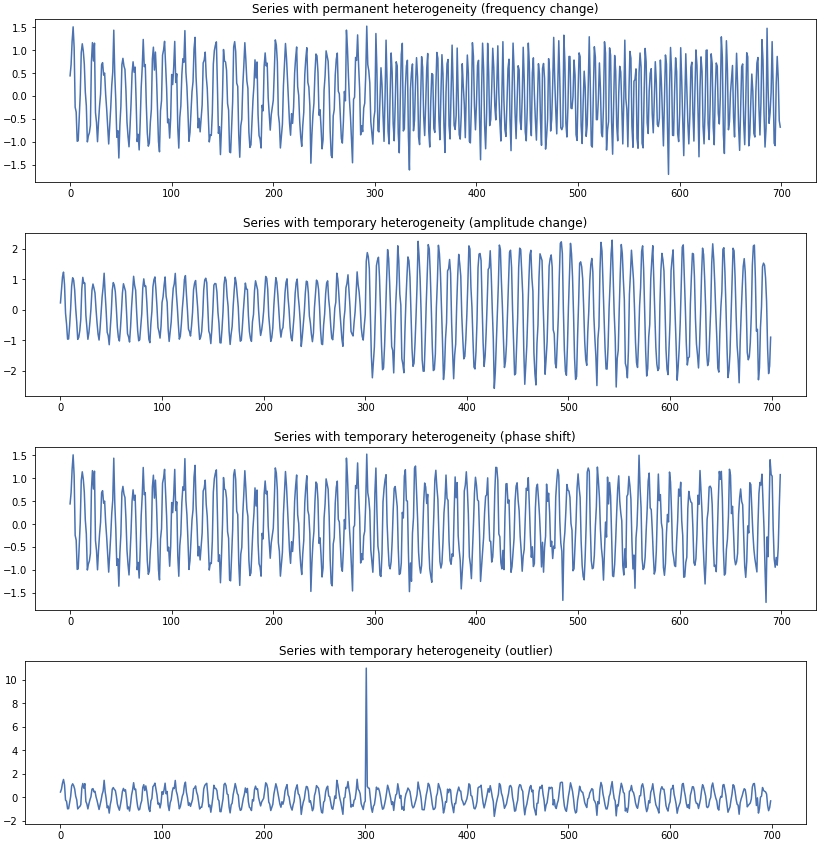
\includegraphics[width=1\linewidth]{seriesNoisedTests}}
	\caption{Временные ряды c шумом.}
	\label{pic:TimeSeriesWithNoise}
\end{figure}

\newpage
\begin{figure}[!hhh]
	\center{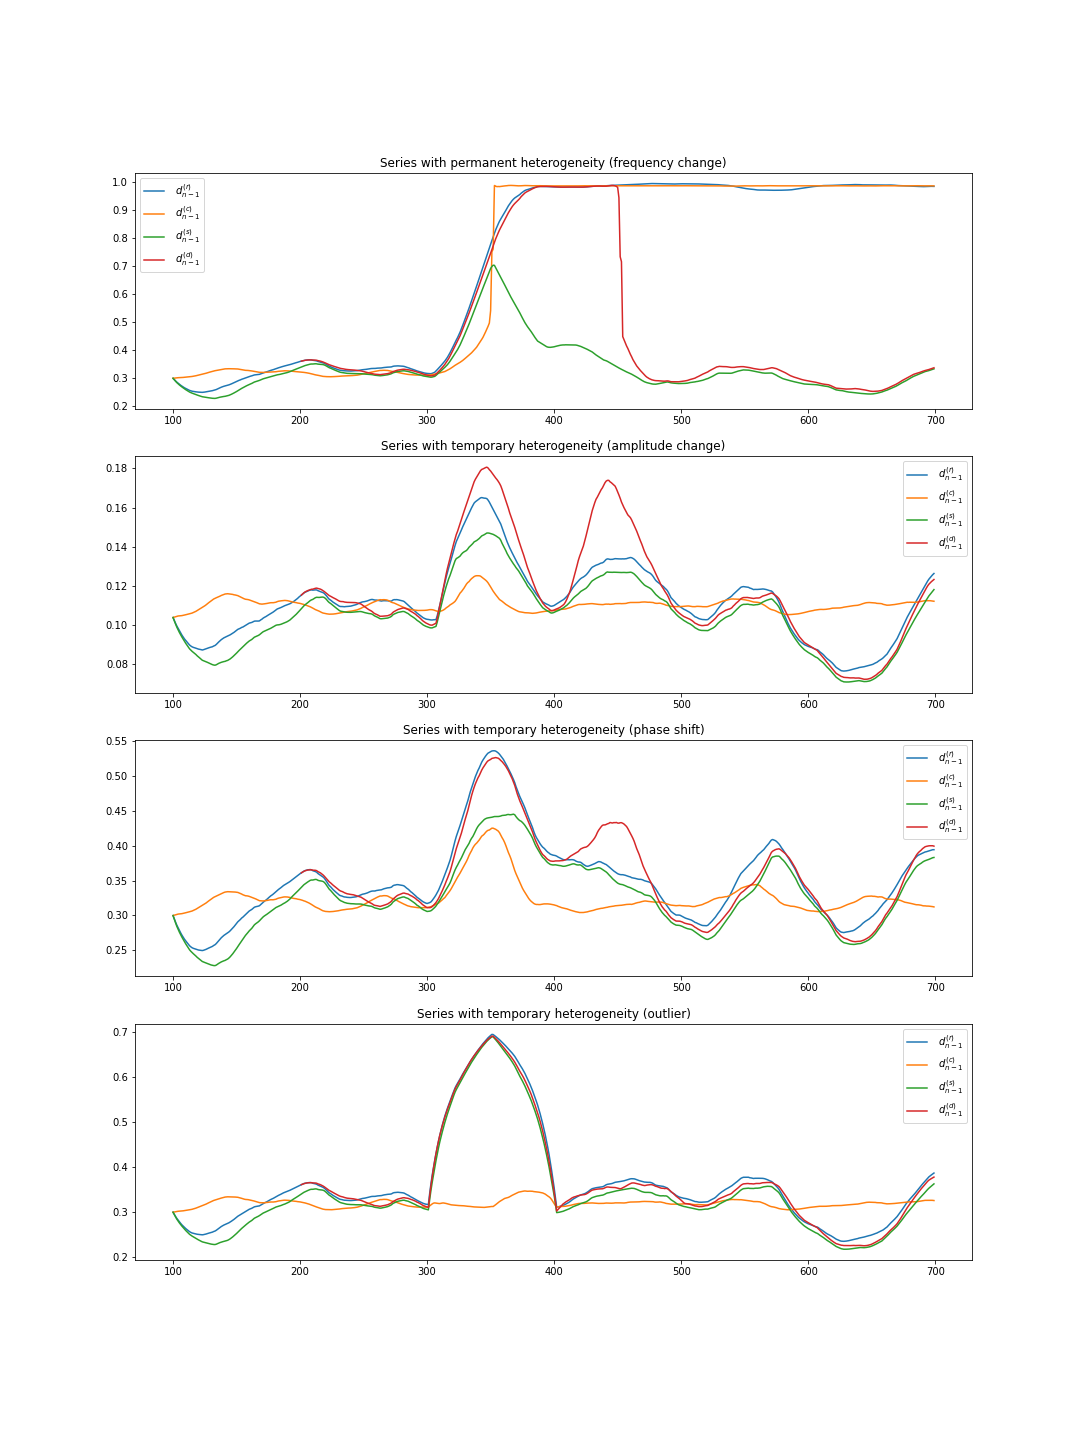
\includegraphics[width=1\linewidth]{detectionNoisedTests}}
	\caption{Функции неоднородности рядов с шумом.}
	\label{pic:HeterFuncsWithNoise}
\end{figure}

\newpage
\begin{table}[!hhh]
	\caption{Характеристики функций неоднородности для постоянной разладки с шумом($\omega_1 \neq \omega_2$).}
	\begin{tabular}{lllllll}
		Row & meanMax & 95 procentile &  & Col & meanMax & 95 procentile \\
		$\#n_{overcome}$ & 200 & 200 &  & $\#n_{overcome}$ & 200 & 200 \\
		$n_{overcome}$ & 312.36 & 311.71 &  & $n_{overcome}$ & 315.69 & 315.32 \\
		$D_Q^{(r)}$ & 0.1949 & 0.1949 &  & $D_Q^{(c)}$ & 0.1979 & 0.1979 \\
		$D_{Q+10}^{(r)}$ & 0.2308 & 0.2308 &  & $D_{Q+10}^{(c)}$ & 0.2010 & 0.2010 \\
		$D_{Q+20}^{(r)}$ & 0.3148 & 0.3148 &  & $D_{Q+20}^{(c)}$ & 0.2140 & 0.2140 \\
		$D_{Q+30}^{(r)}$ & 0.4345 & 0.4345 &  & $D_{Q+30}^{(c)}$ & 0.2379 & 0.2379 \\
		&  &  &  &  &  &  \\
		Sym & meanMax & 95 procentile &  & Diag & meanMax & 95 procentile \\
		$\#n_{overcome}$ & 200 & 200 &  & $\#n_{overcome}$ & 200 & 200 \\
		$n_{overcome}$ & 312.91 & 312.165 &  & $n_{overcome}$ & 309.195 & 308.79 \\
		$D_Q^{(s)}$ & 0.1903 & 0.1903 &  & $D_Q^{(d)}$ & 0.1950 & 0.1950 \\
		$D_{Q+10}^{(s)}$ & 0.2234 & 0.2234 &  & $D_{Q+10}^{(d)}$ & 0.2283 & 0.2283 \\
		$D_{Q+20}^{(s)}$ & 0.2976 & 0.2976 &  & $D_{Q+20}^{(d)}$ & 0.3056 & 0.3056 \\
		$D_{Q+30}^{(s)}$ & 0.4044 & 0.4044 &  & $D_{Q+30}^{(d)}$ & 0.4210 & 0.4210
	\end{tabular}
	\label{tab:PermanentNoisedHeterogeneity}
\end{table}

\newpage
\begin{table}[!hhh]
	\caption{Характеристики функций неоднородности для временной разладки с шумом ($С_1 \neq С_2$).}
	\begin{tabular}{lllllll}
		Row & meanMax & 95 procentile &  & Col & meanMax & 95 procentile \\
		$\#n_{overcome}$ & 200 & 200 &  & $\#n_{overcome}$ & 200 & 200 \\
		$n_{overcome}$ & 308.475 & 308.03 &  & $n_{overcome}$ & 309.07 & 308.88 \\
		$D_Q^{(r)}$ & 0.0564 & 0.0564 &  & $D_Q^{(c)}$ & 0.0578 & 0.0578 \\
		$D_{Q+10}^{(r)}$ & 0.0768 & 0.0768 &  & $D_{Q+10}^{(c)}$ & 0.0612 & 0.0612 \\
		$D_{Q+20}^{(r)}$ & 0.1028 & 0.1028 &  & $D_{Q+20}^{(c)}$ & 0.0735 & 0.0735 \\
		$D_{Q+30}^{(r)}$ & 0.1181 & 0.1181 &  & $D_{Q+30}^{(c)}$ & 0.0861 & 0.0861 \\
		&  &  &  &  &  &  \\
		Sym & meanMax & 95 procentile &  & Diag & meanMax & 95 procentile \\
		$\#n_{overcome}$ & 200 & 200 &  & $\#n_{overcome}$ & 200 & 200 \\
		$n_{overcome}$ & 311.14 & 309.94 &  & $n_{overcome}$ & 305.64 & 305.34 \\
		$D_Q^{(s)}$ & 0.0551 & 0.0551 &  & $D_Q^{(d)}$ & 0.0564 & 0.0564 \\
		$D_{Q+10}^{(s)}$ & 0.0723 & 0.0723 &  & $D_{Q+10}^{(d)}$ & 0.0789 & 0.0789 \\
		$D_{Q+20}^{(s)}$ & 0.0868 & 0.0868 &  & $D_{Q+20}^{(d)}$ & 0.1095 & 0.1095 \\
		$D_{Q+30}^{(s)}$ & 0.0900 & 0.0900 &  & $D_{Q+30}^{(d)}$ & 0.1284 & 0.1284
	\end{tabular}
	\label{tab:TemporaryHeterogeneityNoisedAmplitude}
\end{table}

\newpage
\begin{table}[!hhh]
	\caption{Характеристики функций неоднородности для временной разладки с шумом ($\phi_1 \neq \phi_2$).}
	\begin{tabular}{lllllll}
		Row & meanMax & 95 procentile &  & Col & meanMax & 95 procentile \\
		$\#n_{overcome}$ & 200 & 200 &  & $\#n_{overcome}$ & 200 & 200 \\
		$n_{overcome}$ & 312.08 & 311.395 &  & $n_{overcome}$ & 310.81 & 310.52 \\
		$D_Q^{(r)}$ & 0.1994 & 0.1994 &  & $D_Q^{(c)}$ & 0.1997 & 0.1997 \\
		$D_{Q+10}^{(r)}$ & 0.2313 & 0.2313 &  & $D_{Q+10}^{(c)}$ & 0.2053 & 0.2053 \\
		$D_{Q+20}^{(r)}$ & 0.2978 & 0.2978 &  & $D_{Q+20}^{(c)}$ & 0.2312 & 0.2312 \\
		$D_{Q+30}^{(r)}$ & 0.3672 & 0.3672 &  & $D_{Q+30}^{(c)}$ & 0.2790 & 0.2790 \\
		&  &  &  &  &  &  \\
		Sym & meanMax & 95 procentile &  & Diag & meanMax & 95 procentile \\
		$\#n_{overcome}$ & 200 & 200 &  & $\#n_{overcome}$ & 200 & 200 \\
		$n_{overcome}$ & 313.8 & 312.815 &  & $n_{overcome}$ & 308.79 & 308.355 \\
		$D_Q^{(s)}$ & 0.1948 & 0.1948 &  & $D_Q^{(d)}$ & 0.1993 & 0.1993 \\
		$D_{Q+10}^{(s)}$ & 0.2217 & 0.2217 &  & $D_{Q+10}^{(d)}$ & 0.2277 & 0.2277 \\
		$D_{Q+20}^{(s)}$ & 0.2671 & 0.2671 &  & $D_{Q+20}^{(d)}$ & 0.2874 & 0.2874 \\
		$D_{Q+30}^{(s)}$ & 0.3009 & 0.3009 &  & $D_{Q+30}^{(d)}$ & 0.3599 & 0.3599
	\end{tabular}
	\label{tab:TemporaryHeterogeneityNoisedShifted}
\end{table}

\newpage
\begin{table}[!hhh]
	\caption{Характеристики функций неоднородности для временной разладки с шумом (выброс).}
	\begin{tabular}{lllllll}
		Row & meanMax & 95 procentile &  & Col & meanMax & 95 procentile \\
		$\#n_{overcome}$ & 200 & 200 &  & $\#n_{overcome}$ & 180 & 181 \\
		$n_{overcome}$ & 302.25 & 302.185 &  & $n_{overcome}$ & 311.2389 & 311.0663 \\
		$D_Q^{(r)}$ & 0.1982 & 0.1982 &  & $D_Q^{(c)}$ & 0.2050 & 0.2049 \\
		$D_{Q+10}^{(r)}$ & 0.4814 & 0.4814 &  & $D_{Q+10}^{(c)}$ & 0.2318 & 0.2316 \\
		$D_{Q+20}^{(r)}$ & 0.5929 & 0.5929 &  & $D_{Q+20}^{(c)}$ & 0.2334 & 0.2333 \\
		$D_{Q+30}^{(r)}$ & 0.6555 & 0.6555 &  & $D_{Q+30}^{(c)}$ & 0.2268 & 0.2266 \\
		&  &  &  &  &  &  \\
		Sym & meanMax & 95 procentile &  & Diag & meanMax & 95 procentile \\
		$\#n_{overcome}$ & 200 & 200 &  & $\#n_{overcome}$ & 200 & 200 \\
		$n_{overcome}$ & 302.31 & 302.275 &  & $n_{overcome}$ & 301.845 & 301.795 \\
		$D_Q^{(s)}$ & 0.1935 & 0.1935 &  & $D_Q^{(d)}$ & 0.1980 & 0.1980 \\
		$D_{Q+10}^{(s)}$ & 0.4619 & 0.4619 &  & $D_{Q+10}^{(d)}$ & 0.4855 & 0.4855 \\
		$D_{Q+20}^{(s)}$ & 0.5760 & 0.5760 &  & $D_{Q+20}^{(d)}$ & 0.5971 & 0.5971 \\
		$D_{Q+30}^{(s)}$ & 0.6440 & 0.6440 &  & $D_{Q+30}^{(d)}$ & 0.6598 & 0.6598
	\end{tabular}
	\label{tab:TemporaryHeterogeneityNoisedOutlier}
\end{table}

По результатам видим что в среднем, диагональная функция неоднородности $d_{n-1}^{(d)}$ раньше обнаруживает разладку среди остальных трех, при этом, уступая в скорости возрастания строковой в примерах с постоянной ($\omega_1 \neq \omega_2$) и временной (выброс) разладками. 

\newpage
\subsection{Выводы}

\begin{table}[!hhh]
	\caption{Средние значения характеристик функций обнаружения.}
	\begin{tabular}{lllllll}
		Row & meanMax & 95 procentile \\
		$Mean(\#n_{overcome})$ & 200 & 200 \\
		$Mean(n_{overcome})$ & 308.791 & 308.330 \\
		$Mean(||[D_Q^{(r)},\; D_{Q+10}^{(r)},\; D_{Q+20}^{(r)},\; D_{Q+30}^{(r)}]||_{l2})$ & 0.597 & 0.597 \\
		&  &  \\
		Col & meanMax & 95 procentile \\
		$Mean(\#n_{overcome})$ & 195 & 195.25 \\
		$Mean(n_{overcome})$ & 311.702 & 311.447 \\
		$Mean(||[D_Q^{(c)},\; D_{Q+10}^{(c)},\; D_{Q+20}^{(c)},\; D_{Q+30}^{(c)}]||_{l2})$ & 0.370 & 0.370 \\
		&  &  \\
		Sym & meanMax & 95 procentile \\
		$Mean(\#n_{overcome})$ & 200 & 200 \\
		$Mean(n_{overcome})$ & 310.040 & 309.299 \\
		$Mean(||[D_Q^{(s)},\; D_{Q+10}^{(s)},\; D_{Q+20}^{(s)},\; D_{Q+30}^{(s)}]||_{l2})$ & 0.558 & 0.558 \\
		&  &  \\
		Diag & meanMax & 95 procentile \\
		$Mean(\#n_{overcome})$ & 200 & 200 \\
		$Mean(n_{overcome})$ & 306.368 & 306.070 \\
		$Mean(||[D_Q^{(d)},\; D_{Q+10}^{(d)},\; D_{Q+20}^{(d)},\; D_{Q+30}^{(d)}]||_{l2})$ & 0.595 & 0.595
	\end{tabular}
	\label{tab:AvgResultsNoise}
\end{table}

Явными фаворитами (таблица \ref{tab:AvgResultsNoise}) являются строковая $d_{n-1}^{(r)}$ и диагональная $d_{n-1}^{(d)}$ функции неоднородности. Они обе показывают превосходство над столбцовой $d_{n-1}^{(c)}$ и симметричной $d_{n-1}^{(s)}$ в устойчивости к шуму $\epsilon$, моментом обнаружения разладки $n_{overcome}$ и скорости возрастания значений $[D_Q, D_{Q+10}, D_{Q+20}, D_{Q+30}]$ после момента нарушения однородности $Q$.


\newpage
\chapter{Аналитическая оценка индекса неоднородности при изменении частоты гармоники}
Исходя из заключений прошлой главы о качестве функций обнаружения разладки, далее будем рассматривать элементы строковой функции неоднородности $d_{n-1}^{(r)}$ в качестве индекса неоднородности $ g $.

Рассмотрим ряд $ F_N = (f_0, \dots f_{N-1}) $, причем  
\begin{equation*} 
	f_n = 
	\begin{cases} 
		C_1\sin(2\pi\omega_1 n + \phi_1),\ n \in [0, Q-1] \\ 
		C_2\sin(2\pi\omega_2 n + \phi_2),\ n \in [Q, N-1] 
	\end{cases} 
\end{equation*} 

Обозначим 
$$ F^{(1)} = f_n^{(1)}|_{n=0}^{B-1}, $$
$$ F^{(2)} = f_n^{(2)}|_{n=0}^{T-1}, $$
$$X_l^{(2)} = (f_{l}^{(2)}, \dotsc, f_{l+L-1}^{(2)})^\mathrm{T}, \;\;\; 0 \leq l < K_2.$$

В обозначениях выше, $ F^{(1)} $ - некий подряд ряда $ F_N $ длины $ B $, целиком лежащий в промежутке от начала ряда до точки разладки $ Q $, а  $ F^{(2)} $ - некий подряд ряда $ F_N $ длины $ T $, целиком лежащий в промежутке от точки разладки $ Q $ до конца ряда $ F_N $. 


В соответствии с формулой (2.1), индекс неоднородности задается как:
$$ g(F^{(1)}; F^{(2)}) = 1 - \frac{\sum\limits_{l=0}^{K_2-1}\;\sum\limits_{i=0}^{r-1}\langle X_l^{(2)}, U_i^{(1)}\rangle^2}{\sum\limits_{l=0}^{K_2-1}\|X_l^{(2)}\|^2} = 1 - z(F^{(1)}; F^{(2)}),  $$

где $ z(F^{(1)}; F^{(2)}) $ --- индекс однородности.

В данной главе будем предполагать $ \omega_1 \neq \omega_2;\; C_1 = C_2 $. Для простоты зададим амплитуды $ C_1 = C_2 = 1 $.

Попробуем аналитически упростить данную формулу, чтобы явно увидеть, как разности частот ряда до и после разладки влияют на значения $ g $.

\section{Вычисление индекса однородности}
\subsection{Знаменатель}
Начнем со знаменателя $\sum\limits_{l=1}^{K_2}\|X_l^{(2)}\|^2$, а точнее, с квадрата нормы $\|X_l^{(2)}\|^2$. Оценим его:

$$ \|X_l^{(2)}\|^2 = \sum\limits_{i=1}^{L}(X_{l}^{(2)})_i^2 \approx \int\limits_{0}^{L}\sin^2{(2\pi\omega_2 y + \psi_l)}dy = \frac{L}{2} - \frac{\sin(4\pi L\omega_2 + \psi_l) - \sin(2\psi_l)}{8\pi\omega_2} \approx \frac{L}{2}, $$
где $ \psi_l $ формируется из $ \phi_2 $ и сдвига, порождаемого номером вектора вложения.

Отсюда $\sum\limits_{l=1}^{K_2}\|X_l^{(2)}\|^2 \approx K_2\cdot\frac{L}{2}$.


\subsection{Числитель}
$$ \sum\limits_{l=1}^{K_2}\;\sum\limits_{i=1}^{r}\langle X_l^{(2)}, U_i^{(1)}\rangle^2 = 
\sum\limits_{l=1}^{K_2}\;\left ( \langle X_l^{(2)}, U_1^{(1)}\rangle^2 + \langle X_l^{(2)}, U_2^{(1)}\rangle^2 \right ) = $$
$$ =  \sum\limits_{l=1}^{K_2}\; \left [ \left (\sum\limits_{j=1}^{L}(X_{l}^{(2)})_j\cdot (U_{1}^{(1)})_j\right )^2 + \left ( \sum\limits_{j=1}^{L}(X_{l}^{(2)})_j\cdot (U_{2}^{(1)})_j\right )^2 \right ].$$

Рассмотрим $ U_{1}^{(1)} $ и $U_{2}^{(1)} $. В силу задания ряда, базисом $ U_{1}^{(1)} $ и $U_{2}^{(1)} $ пространства $ \mathfrak{L}_r^{(1)} $, порожденного элементами $ f_n^{(1)} = \sin(2\pi\omega_1 n + \phi_1) $ являются некие нормированные $ \sin(2\pi\omega_1 n + \psi) $ и $ \cos(2\pi\omega_1 n + \psi) $.

Пусть $ p_1 = \sin(2\pi\omega_1 n + \psi) $, $ p_2 = \cos(2\pi\omega_1 n + \psi) $. Вычислим нормы $ p_1 $ и $ p_2 $ для поиска $ U_{1}^{(1)} $ и $U_{2}^{(1)} $. 
По аналогии со знаменателем индекса однородности (п. 5.1.1.), $ \|p_1\| = \|p_2\| \approx \sqrt{\frac{L}{2}} $, откуда $ U_{1}^{(1)} = \frac{\sin(2\pi\omega_1 n + \psi)}{\sqrt{L/2}} $, $ U_{2}^{(1)} = \frac{\cos(2\pi\omega_1 n + \psi)}{\sqrt{L/2}} $.

Пусть  
$$ I_l =  \left (\sum\limits_{j=1}^{L}(X_{l}^{(2)})_j\cdot (U_{1}^{(1)})_j\right )^2, $$
$$ J_l =  \left (\sum\limits_{j=1}^{L}(X_{l}^{(2)})_j\cdot (U_{2}^{(1)})_j\right )^2, $$
$$ a = \omega_1 + \omega_2,\ b = \omega_1 - \omega_2. $$

Тогда
$$ I_l \approx \left( \int\limits_{0}^{L}\sin(2\pi\omega_2 y + \psi_l) \cdot \frac{\sin(2\pi\omega_1 y + \psi)}{\sqrt{L/2}}dy \right)^2 = $$
$$ = \frac{2}{L} \left(\int\limits_{0}^{L}\sin(2\pi\omega_2 y + \psi_l) \cdot \sin(2\pi\omega_1 y + \psi)dy\right )^2 = $$
$$ = \frac{2}{L} 
\left(  
\frac{\sin(2\pi Lb + \psi - \psi_l) - \sin(\psi - \psi_l)}{4\pi b} - \frac{\sin(2\pi La + \psi + \psi_l) - \sin(\psi + \psi_l)}{4\pi a}
\right)^2. $$



$$ J_l \approx \left(\int\limits_{0}^{L}(\sin(2\pi\omega_2 y + \psi_l) \cdot \frac{\cos(2\pi\omega_1 y + \psi)}{\sqrt{L/2}})dy\right)^2 = $$
$$ = \frac{2}{L}\left(\int\limits_{0}^{L}(\sin(2\pi\omega_2 y + \psi_l) \cdot\cos(2\pi\omega_1 y + \psi))dy\right )^2 = $$
$$ = \frac{2}{L} 
\left(  
\frac{\cos(2\pi Lb + \psi - \psi_l) - \cos(\psi - \psi_l)}{4\pi b} - \frac{\cos(2\pi La + \psi + \psi_l) - \cos(\psi + \psi_l)}{4\pi a}
\right)^2. $$


Предположим $ \psi = \psi_l = 0 $, тогда
$$ I_l \approx \frac{2}{L} \left(  \frac{\sin(2\pi Lb)}{4\pi b} - \frac{\sin(2\pi La)}{4\pi a}   \right)^2. $$
$$ J_l \approx \frac{2}{L} \left(  \frac{\cos(2\pi Lb) - 1}{4\pi b} - \frac{\cos(2\pi La) - 1}{4\pi a}  \right)^2. $$


С учетом предположения выше, получаем:

$$ \sum\limits_{l=1}^{K_2}\;\sum\limits_{i=1}^{r}\langle X_l^{(2)}, U_i^{(1)}\rangle^2 \approx K_2 \cdot \left [ I_l + J_l \right] = $$
$$ = \frac{K_2 \cdot 2}{L} \cdot \left[ \left(  \frac{\sin(2\pi Lb)}{4\pi b} - \frac{\sin(2\pi La)}{4\pi a}   \right)^2 + \left(  \frac{\cos(2\pi Lb) - 1}{4\pi b} - \frac{\cos(2\pi La) - 1}{4\pi a}  \right)^2 \right] $$


\section{Индекс неоднородности}
Собирая все вместе, получаем:

$$ g(F^{(1)}; F^{(2)}) = 1 - \frac{\sum\limits_{l=0}^{K_2-1}\;\sum\limits_{i=0}^{r-1}\langle X_l^{(2)}, U_i^{(1)}\rangle^2}{\sum\limits_{l=0}^{K_2-1}\|X_l^{(2)}\|^2} \approx $$
$$ \approx 1 - \frac{\frac{K_2 \cdot 2}{L} \cdot \left[ \left(  \frac{\sin(2\pi Lb)}{4\pi b} - \frac{\sin(2\pi La)}{4\pi a}   \right)^2 + \left(  \frac{\cos(2\pi Lb) - 1}{4\pi b} - \frac{\cos(2\pi La) - 1}{4\pi a}  \right)^2 \right]}{K_2\cdot\frac{L}{2}} = $$
$$ 1 - \frac{\left[ \left(  \frac{\sin(2\pi Lb)}{4\pi b} - \frac{\sin(2\pi La)}{4\pi a}   \right)^2 + \left(  \frac{\cos(2\pi Lb) - 1}{4\pi b} - \frac{\cos(2\pi La) - 1}{4\pi a}  \right)^2 \right]}{\frac{L^2}{4}}, \eqno(5.1)$$
при условии $ \psi = \psi_l = 0 $.

\section{Проверка точности аппроксимации}
При сравнении индекса неоднородности, вычисленного классическим способом и аналитически упрощенным, результаты оказались довольно похожи, причем при $L \rightarrow \infty $ оба значения сходятся друг к другу. Все тесты доступны в \textbf{гитхаб}\footnote{https://github.com/Loulaan/researchWork} репозитории в файле \textbf{Analytical.ipynb}\footnote{https://github.com/Loulaan/researchWork/blob/main/Analytical.ipynb}.



\subsection{Одинаковые частоты}
Пусть $ N = 700,\; Q = 301,\; B = 100,\; T = 100 $. 
Зададим $w1 = \frac{1}{10},\; w2 = \frac{1}{10},\; L = 60$. При одинаковых частотах значения индексов неоднородности должны быть равны $ 0 $. Действительно, по определению $ g $ пространство $ \mathfrak{L_r} $, порожденное рядом $ F_N $ является одним и тем же для любых подрядов $ F^{(1)} $ и $ F^{(2)} $ ряда $ F_N $ так как структура ряда не менялась.
Проверяя этот теоретический факт на практике, получили также $ 0 $.

\subsection{$L\omega_1$ и $L\omega_2 $ целые, $\omega_1 \neq \omega_2 $}
Еще один теоретический факт: 

При целых $L\omega_1$ и $L\omega_2 $ индекс однородности $ z $ обращается в 0. Действительно, в силу построения ряда (гармоника, описываемая синусом с какими-то фиксированными параметрами), скалярное произведение частей исходного ряда по целому периоду на элементы базиса (ортогональные друг другу) обращают числитель в 0, следовательно индекс неоднородности $ g $ всегда равен $ 1 $, что наблюдается на практике.


\subsection{Предположения об $ L $}

Зафиксируем $ w2 = \frac{1}{11} $ и будем изменять $ L $. В таблице \ref{tab:L_vs_g_c_vs_g_a} показаны значения индексов неоднородности при разных $ L $.

\begin{table}[!hhh]
	\centering
	\caption{Зависимость значений индекса неоднородности, вычисленного классическим $ g_c $ и аналитически упрощенным $ g_a $ способами от величины $ L $.}
	\begin{tabular}{lll}
		$ L $  & $ g_c $     & $ g_a $       \\
		$ 50 $ & $ 0.518365 $ & $ 0.562352 $ \\
		$ 80 $ & $ 0.890753 $ & $ 0.891823 $ \\
		$ 90 $ & $ 0.955854 $ & $ 0.953909 $
	\end{tabular}
\label{tab:L_vs_g_c_vs_g_a}
\end{table}


Чтобы наглядно продемонстрировать стремление значений друг к другу, посмотрим на Рис. \ref{pic:g_c_vs_g_a_from_L}.
\begin{figure}[!hhh]
	\center{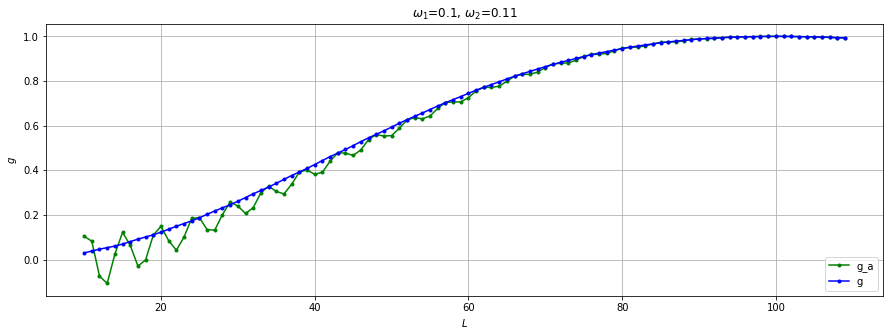
\includegraphics[width=1.0\linewidth]{dynamics_L}}
	\caption{Зависимость индексов $ g_c $ и $ g_a $ от $ L $.}
	\label{pic:g_c_vs_g_a_from_L}
\end{figure}

Исходя из кривых на Рис. \ref{pic:g_c_vs_g_a_from_L}, $ g \rightarrow 1 \text{ при } L \rightarrow \infty$ --- справедливо для обеих формул $ (2.1), \; (5.1) $. 

Данный эксперименты подтверждает что при достаточно больших $ L $ аппроксимация индекса неоднородности выведенной аналитической формулой $ (5.1) $ точна.

\subsection{Разность $\omega_1$ и $ \omega_2 $}
\newtheorem{statement}{Утверждение}

\begin{statement}
	Чем сильнее разница $ \omega_1 $ и $ \omega_2 $, тем проще определить разладку.
\end{statement}

Иными словами, чем больше разница $ \omega_1 $ и $ \omega_2 $, тем быстрее индекс неоднородности $ g $ переходит в $ 1 $.

Пусть $ \omega_1 \geq \omega_2, \; \omega_2 \rightarrow \omega_1 $. Аналитически, в пределе $ a = 2\omega_1,\; b = 0 $. Тогда $$ g = 1 - \frac{(\frac{L}{2} - \frac{\sin(4\pi L\omega_1)}{8\pi\omega_1} + \frac{\omega_2}{2\pi\omega_1^2})^2}{\frac{L^2}{4}} \approx 1 - \frac{(\frac{L}{2})^2}{\frac{L^2}{4}} = 1 - 1 = 0 $$

При проверке данного предположения, получились значения $ g_c = 0.0,\; g_a = 3.330669e-16 \approx 0 $.

Посмотрим на график зависимости $ g $ от $ \omega_2 $ при фиксированном $ \omega_1 = \frac{1}{10} $.

\begin{figure}[!hhh]
	\center{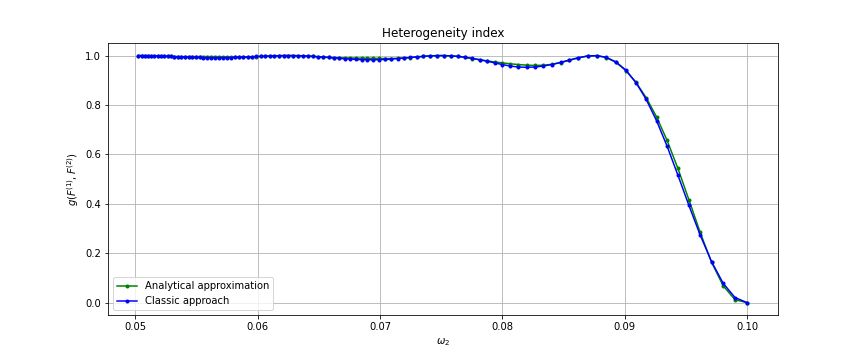
\includegraphics[width=1.0\linewidth]{dynamics_w2}}
	\caption{Зависимость индексов $ g_c $ и $ g_a $ от $ \omega_2 $.}
	\label{pic:g_c_vs_g_a_from_w_2}
\end{figure}

По кривым на Рис. \ref{pic:g_c_vs_g_a_from_w_2} видим, что чем ближе частоты друг к другу, тем ближе индекс неоднородности к $ 0 $, и, соответственно, чем дальше, тем ближе $ g $ к $ 1 $, что подтверждает \textbf{Утверждение 1.}



\newpage
\chapter*{Заключение}
\addcontentsline{toc}{chapter}{Заключение}

В данной работе были рассмотрены и сравнены функции обнаружения неоднородности в синусоидальных временных рядах с неоднородностями, заданными изменением частоты, амплитуды, фазовым сдвигом и выбросом. 

Также был тщательно рассмотрен и аналитически упрощен индекс неоднородности $ g(F^{(1)}, F^{(2)}) $. Для аналитической аппроксимации были приведены тесты, доказывающие эквивалентность классической и упрощенной формул для $ g $.




\begin{thebibliography}{3}
	\bibitem{TSStructure}
	Golyandina, N., Nekrutkin, V., \& Zhigljavsky, A. (2001). Analysis of time series structure: SSA and related techniques. Chapman \& Hall/CRC.
\end{thebibliography}

	
\end{document}